\documentclass[a4paper,11pt]{article}
\usepackage{graphicx}
\usepackage[T1]{fontenc}
\usepackage[latin1]{inputenc}
\usepackage{graphicx}
\usepackage{titlesec}
\usepackage{xcolor}
\usepackage{amsfonts}
\usepackage{algorithm}
\usepackage{wrapfig}
\usepackage{algpseudocode}
\usepackage{wrapfig}
\usepackage{svg}
\usepackage{amssymb}
\usepackage{floatflt,epsfig}
\usepackage{subfigure}
\usepackage{multirow}
\usepackage{glossaries}
\usepackage{booktabs}
\newtheorem{theorem}{Theorem}
\newtheorem{lemma}{Definition}
\newtheorem{proposition}{Proposition}
\newtheorem{proof}{Proof}
\usepackage{tikz}
\tikzstyle{mybox} = [draw=black, thin, rectangle, rounded corners, inner ysep=5pt, inner xsep=5pt, fill=orange!20]

\usepackage[a4paper, top=2cm , bottom=2cm , right=1.5cm , left=1.5cm ]{geometry}

\begin{document}
    
    \title{
        \linespread{0.3}
        \vspace{-2.5cm}
        \textbf{
        {\large{MODELING AND CONTROL OF CPSs}  - \Large {Project activity report (Part II)}}\\
        {\Large \underline{\textsf{Distributed control of a multi-agents magnetic levitation system}}}
        %{\Large{Project Activity Report}}
        }
        \vspace{-0.5em}
    }
    \author{
        \textit{
            \normalsize 
        Lorenzo AGHILAR} \text{(334086)},
        \textit{Carlo MIGLIACCIO} (332937), 
        \textit{Federico PRETINI} (329152)}
    
    \date{}

    \clearpage\maketitle
    \thispagestyle{empty}
    \vspace{-2em}

    {
        \centering
        \noindent
        \textsf{        
            In this second part of the report the objective is to present the design of a dynamic cooperative (distributed) regulator for a multi-agent systems composed of 7 magnetic levitator which are organized in a way that there is a leader node and six followers. Since the physical quantity are not directly measurable an observer has to be employed.} \textbf{\color{red} This part can be left here} 
    }
   
    \section*{Brief theoretical introduction}
    \textsf{
    In this part the focus is introducing the setting in which we have to work, definition of the structures for the leader and the follower...Introduction of the specific type of system to be controlled (magnetic levitator).
    How we model the communication network? (matrices $\mathcal{A}, D, G, L$)...
    What is the structure of the control law? What is the way in which the controller can be implemented?\\
    Few words on the estimation approaches can be used in the framework of control of Multi-Agent systems.}

    \section*{Network structures}
    \texttt{See the notes about this point in the folder for more details...}\\
    \textsf{
    Briefly speaking some considerations are given on the values of the matrix $A_c$ of the global estimation error dynamics, this is related directly to $c(L+G)$ which depends on the graph structure. An analysis on the eigenvalues is provided, another parameter is considered is the \textbf{settling time}.\\
    I found in the IEEE portal some papers about the relationship between convergence rate and network structure, but they used some results on the so-called \textit{algebraic connectivity}...}
    \begin{figure}[h]
        \centering
        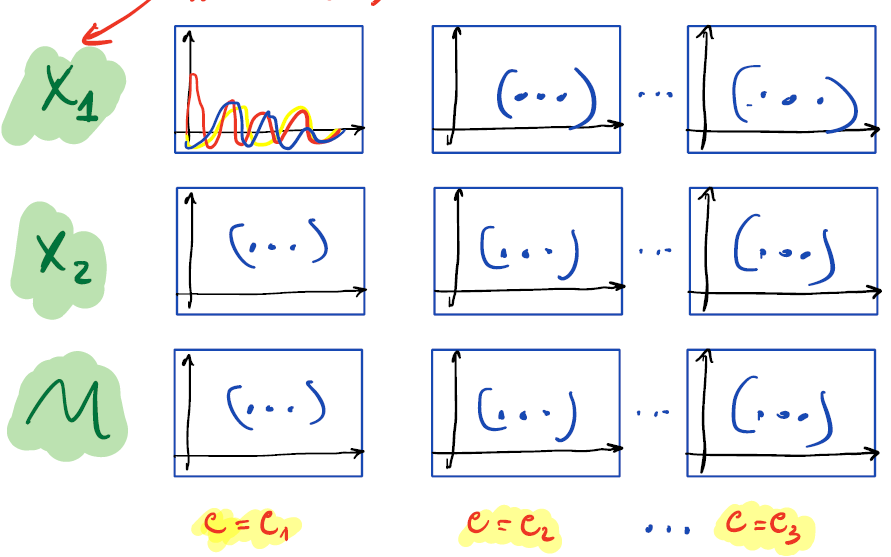
\includegraphics[scale=0.6]{img/figCoupling.png}
        \caption{Possible presentation of the results (coupling gain)}
    \end{figure}
    \section*{Effect of the coupling gain}
    \textsf{
    Selection of a certain number of $c$ which satisfy the condition imposed by the \textbf{Theorem 1}. What is the limit to this choise? We know that the $c$ parameter enters directly in the control law $u_i$ which is given tipically by actuators. These are surely subject to saturation. \textsf{For this point the book "Laboratorio Sperimentale di Automatica - Greco, Spagnolo" can be used, more specifically the chapter that is related to "Magnetic Levitator"}.
    \subsection*{Useful graphs}
    Plots for leader and follower nodes for the variables $x_1, x_2, u$. The analysis can be conducted for each one of the two approaches by using: 
    \begin{enumerate}
        \itemsep-0.2em
        \item Constant reference to generate for the leader, to follow for the others; 
        \item no noise is considered
        \item Fixed $Q, R$, for example $Q=I_2$, $R=1$ since in this part it is not relevant focus the attention on the weighting matrices.
        \item Repeat this steps for the second approach
    \end{enumerate} }



    \section*{Effect of $Q, R$ weighting matrices}
    \textsf{
    \textsf{\color{red} [no noise, $(c, K, F)$ fixed]}
    Try to change the relative value of the weighting matrices. It is remarkable that they are associated to the solution of the \textit{local optimal LQ problem}. Several choices can be done: for example (i) Q=R (ii) entries in Q less than entries in R and viceversa.
    The type of analisys could be conducted is the plot of $x_1, x_2, u$ for the different choices of Q, R. For an estimation method and for the other. \\
    Remember that: $Q$ is related to the energy of the state of the system; $R$ is related to the energy of the input, that is the \textbf{command effort}.}

    \begin{figure}[h]
        \centering
        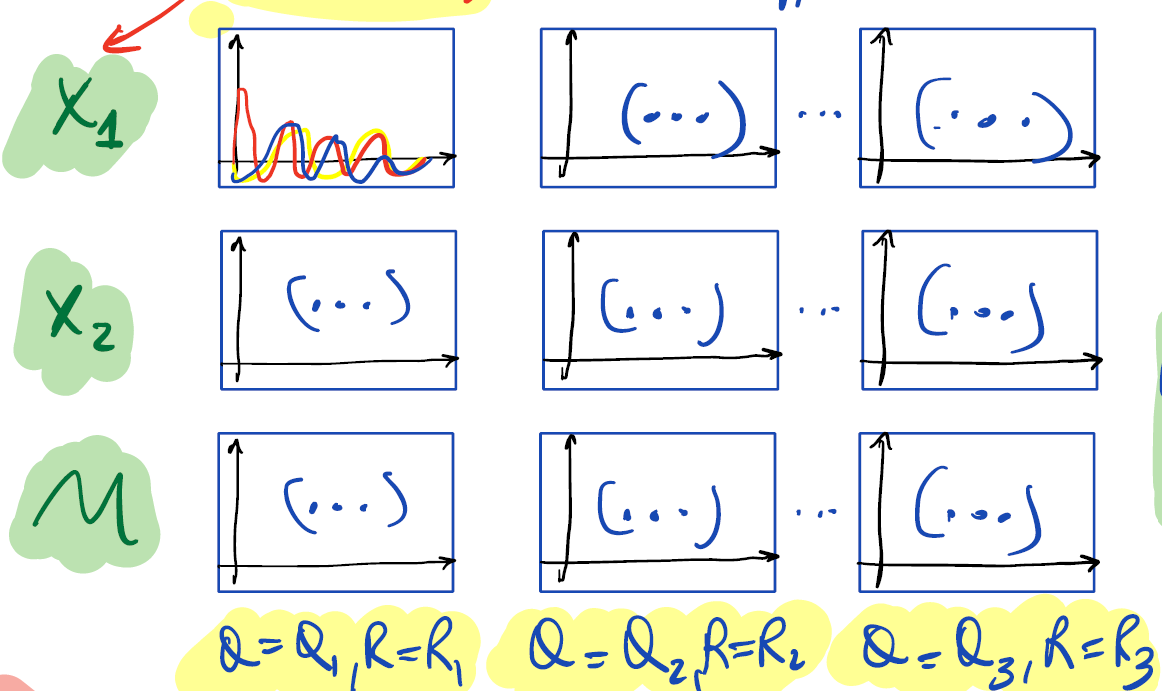
\includegraphics[scale=0.5]{img/figQR.png}
        \caption{Possible presentation of the results (weighting matrices)}
    \end{figure}

    \section*{Effect of measurement noise}
    \textsf{
    What is the effect of \textbf{measurement noise}? Measurement noises are fundamental to be taken into account, they always are present. In this part we wonder which are the performances in case of measurement noise for the first approach, for the second approach.     \\
    In particular: 
    \begin{enumerate}
        \item How the noise enters in the estimation algorithm (in the first and second approach)? By doing calculations, the conclusion is that: 
        \begin{itemize}
            \item In the first approach (local observer) the error enters in the estimation algorithm as an additive term $cFd_p^{(i)}$, where $d_p$ is the measurement noise.
            \item In the case that a cooperative observer is employed there is an additive term to consider {$$cF\sum_{j=1}^N a_{ij}(d_p^j-d_p^i)+g_0(d_p^0 - d_p^i)$$}
        \end{itemize}
        \item Within the same approach consider different situations: (i) only the leader node is affected by measurement noise, (ii) leader + some agents, (iii) leader + all the agents.
        \item Repeat the analysis for the first and second approach.
        At this point: 
        \begin{enumerate}
            \itemsep-0.2em
            \item What is the best approach when there are measurement noises?
            \item What we can do in order to reduce their effect?
        \end{enumerate}
    \end{enumerate}}

    \begin{figure}[h]
        \centering
        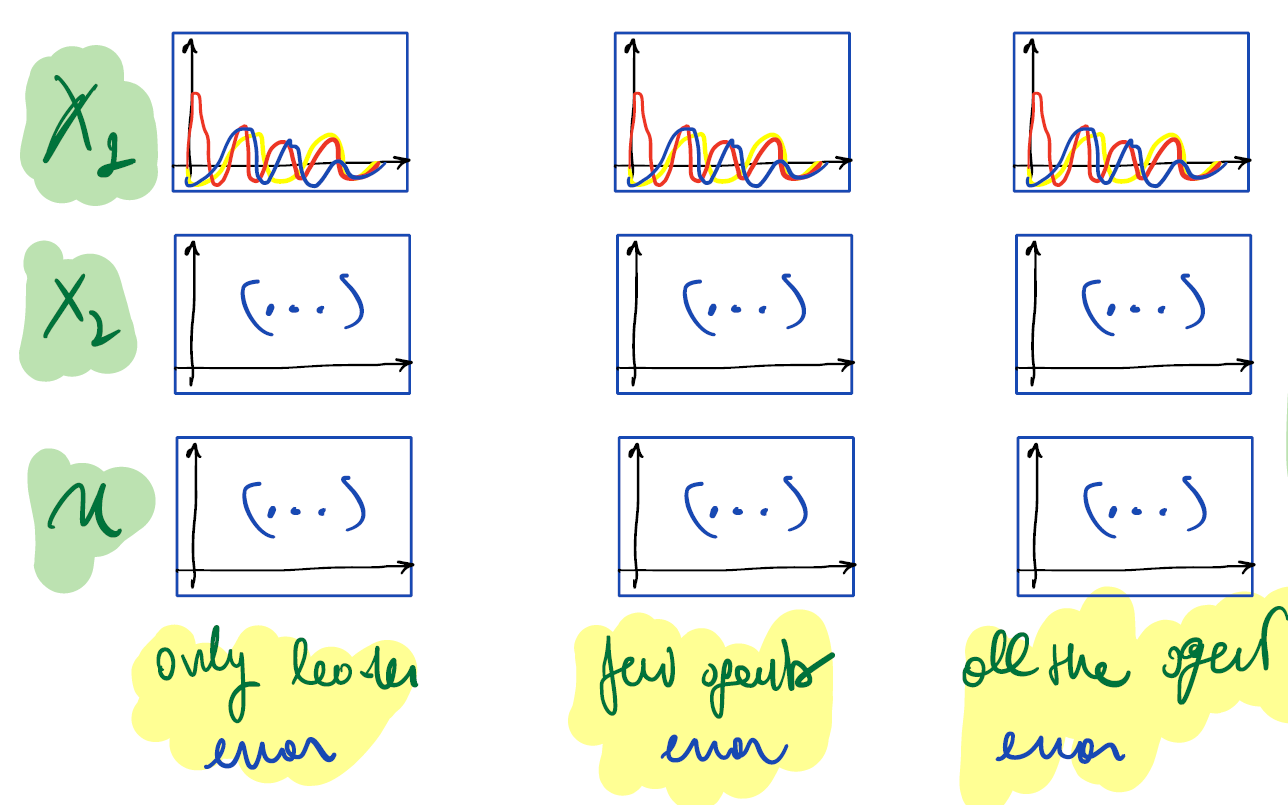
\includegraphics[scale=0.4]{img/figNoise.png}
        \caption{Possible presentation of the results (measurement noise)}
    \end{figure}
\end{document}